\documentclass[journal]{vgtc}                % final (journal style)

%% These few lines make a distinction between latex and pdflatex calls and they
%% bring in essential packages for graphics and font handling.
%% Note that due to the \DeclareGraphicsExtensions{} call it is no longer necessary
%% to provide the the path and extension of a graphics file:
%% 
\includegraphics{diamondrule} is completely sufficient.
%%
\ifpdf%                                % if we use pdflatex
  \pdfoutput=1\relax                   % create PDFs from pdfLaTeX
  \pdfcompresslevel=9                  % PDF Compression
  \pdfoptionpdfminorversion=7          % create PDF 1.7
  \ExecuteOptions{pdftex}
  \usepackage{graphicx}                % allow us to embed graphics files
  \DeclareGraphicsExtensions{.pdf,.png,.jpg,.jpeg} % for pdflatex we expect .pdf, .png, or .jpg files
\else%                                 % else we use pure latex
  \ExecuteOptions{dvips}
  \usepackage{graphicx}                % allow us to embed graphics files
  \DeclareGraphicsExtensions{.eps}     % for pure latex we expect eps files
\fi%

%% it is recomended to use ``\autoref{sec:bla}'' instead of ``Fig.~\ref{sec:bla}''
\graphicspath{ {pictures/} } % where to search for the images

\usepackage{microtype}                 % use micro-typography (slightly more compact, better to read)
\usepackage{hyperref}
\usepackage{listings}
\usepackage{cite}

\PassOptionsToPackage{warn}{textcomp}  % to address font issues with \textrightarrow
\usepackage{times}                     % we use Times as the main font
\renewcommand*\ttdefault{txtt}         % a nicer typewriter font

%% declare the category of your paper, only shown in review mode
\vgtccategory{Research}

\title{How NBA Player Salaries Relate to Individual and Team Performance: Using Visualizations to Maximize a Team's Success}

\author{Alex Hoffer, Austin Nguyen, Prathveer Rai}

\abstract{
This paper attempts to describe how an NBA player's salary can be beneficial or detrimental to their team based on their performance in several statistical categories. This serves as a useful starting point for front office professionals employed by NBA teams who wish to make reasoned judgments about whether they should extend a player's contract or let them walk into free agency. After all, statistics in NBA basketball have become nuanced and sophisticated in the past decade, and teams such as the San Antonio Spurs have embraced their use and excel as a result. We believe that visualizations are the best method for truly understanding the effectiveness of an NBA player in the context of their salary since when these statistics are merely presented in their numerical form, people who are not mathematical experts (such as NBA General Managers, who are responsible for offering contracts to players) may not grasp the conclusion, or even worse, they may get the wrong impression about a certain player. Specifically, we believe that the radar chart is the most appropriate type of visualization to achieve this effect, since there are multiple statistical categories being judged by their relation to salary, which means it is essential that the user is able to see how far out edges extend within each category so they can conveniently visually compare how far out the edge pertaining to the salary is in relation to these statistics, giving them an indication of whether the player is worth their price.}




\date{\today}

\renewcommand{\manuscriptnotetxt}{}

\vgtcinsertpkg

\begin{document}

\maketitle

\section{Introduction}
Basketball players employed by the National Basketball Association (NBA) make a tremendous amount of money. Their agents negotiate with the general managers of professional teams in order to get a salary that they think their performance warrants. Unlike professional sports leagues like Major League Baseball (MLB), though, NBA teams have a \emph{salary cap}, which is a limit to the amount of money they can spend to field a 15-man teamof \$102 million. This means that it is within each NBA team's interests to pay each player in, the average case, the exact salary which fairly corresponds to their on-court performance and, in the best case scenario for the team, a salary that is as low as possible for a player that is extremely good. A good example of the latter case being beneficial to a team is Stephen Curry of the Golden State Warriors, who gets paid x/year, and yet is a two-time MVP who is commonly considered one of the best players of all time. This low salary allowed the Warriors to spend money on acquiring Kevin Durant, another MVP, for a max salary. 
\par Thus, this paper describes the process of our visualizations of the radar chart variety of specific players we believe are beneficial to observe in this way, since it has the capacity to captivate general managers of NBA teams into making the most reasoned decisions about who to sign and who to let walk in free agency. The paper will consist of several sections to achieve this effect, including the related visualizations we have found, the method we used to generate our visual computations, our programming implementation of these concepts, our results and their impact, and what we can conclude from our project and what future visualizations in this realm should address. 

\section{Related Work}
The use of spider charts to visualize NBA statistics is somewhat prevalent in the realm of entertainment, but not in information visualization research. 
\subsection{In Information Visualization Research}
Historically, academic publications in information visualization rarely tackle the topic of sports, much less spider charts devoted to NBA player statistics and their salary. However, over the past several years, this trend has begun to reverse, with conferences such as the IEEE VIS sponsoring workshops on sports data visualization, though the majority of these visualizations regard sports such as football, soccer, and baseball. Nevertheless, it is important for our purposes to survey the few visualizations within this subcategory of information visualization pertaining to the NBA that are present in academic research. \cite{chu}, a paper that introduces an interactive shot chart tool that allows the user to choose a player and see on a virtual basketball court the physical areas on the court where they perform best, presents the idea of using visualization to enhance our assessments of NBA players' in-game performances, but does not describe how tools like this could be used by NBA executives to make reasoned decisions about players' salaries. \cite{chen} proposes a new way of presenting post-game information, gravitating away from webcasts and towards "season level, game level, and session level" visualizations, but the purpose of this work is to augment the NBA fan's experience and, while this work does include some visualizations of performances that are relevant to our research, the purpose of such visualizations is for entertainment consumption and not for the maximization of team success. \cite{pagno} includes some visualizations that are similar to the ones we present in this work, including spider charts with steals, points, rebounds, assists, blocks, and turnovers as graph points of players such as Steve Nash, Deron Williams, and Rajon Rondo. However, these visualizations do not include player salary, which means they do not explore the financial implications of player performance that come in handy when making player personnel decisions. \cite{reyna} uses line graphs and bar graphs to visualize and compare team performances, but provides no application of the importance of such visualizations to executive decision making nor does it provide visualizations of individual player performance. A compelling sequence of different sports visualizations can be found courtesy of the Information Interfaces team at Georgia Tech University. One interactive visualization of NBA player and team data by this team, a snapshot of which is included below, was particularly influential to the software development necessary for our project since it was the only open source visualization of NBA data.
\begin{figure}[h]
\caption{A snapshot of an interactive visualization of basketball data.}
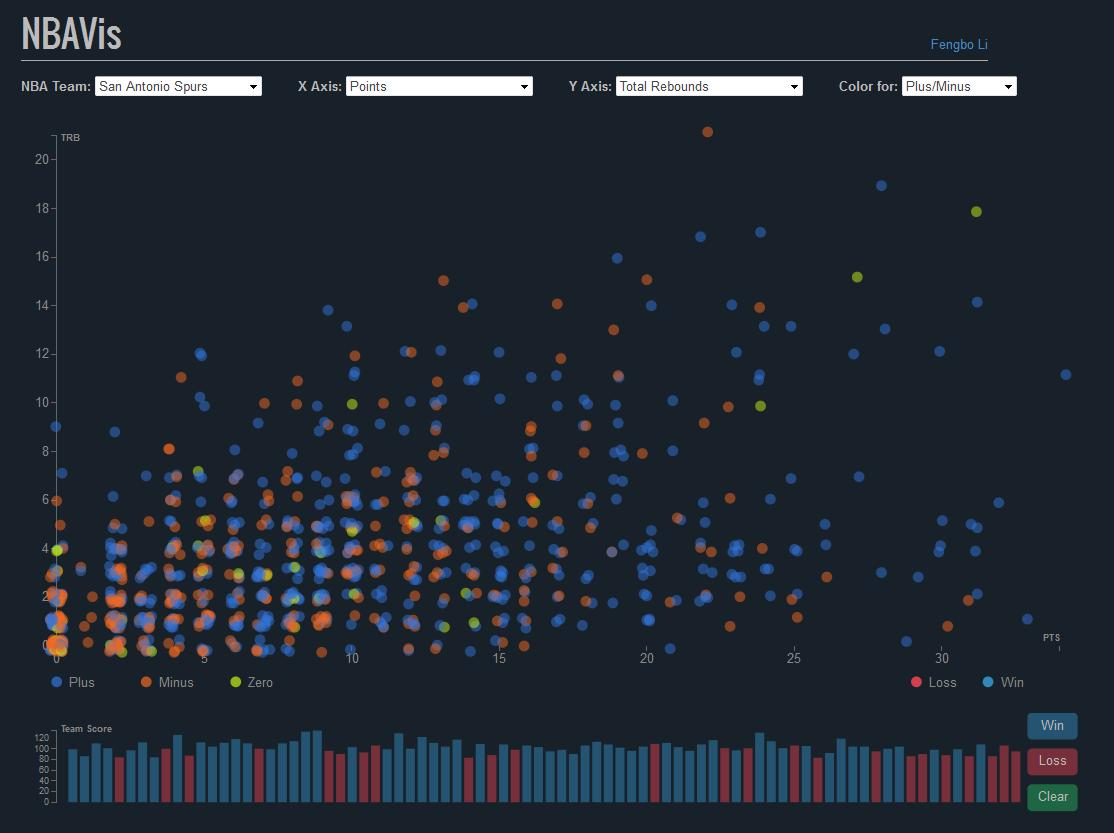
\includegraphics[width=\linewidth]{georgiatech.jpg}
\end{figure}
\subsection{In Entertainment}



\section{Method/Computational Model}
\subsection{Method Overview}
\subsection{Stage 1}
\subsection{Stage n}
\subsection{Parameters}
\subsection{Figures and Images}
\subsection{Enhancements}
\section{Implementation}
\section{Results and Performance}
\subsection{Results}
\subsection{Performance Analysis}
\subsection{Movies and Supplementary Material}
\section{Application Paper}
\section{Conclusions and Future Work}

\newpage
\bibliographystyle{abbrv-doi}
\bibliography{template}

\end{document}

